\section{\ref{algo:sa} Algorithm}

One of the main limitations of the \ref{algo:htf} Algorithm is that when the number of counters is in the same order of the number of HH flows, even after retracting the frontier, the algorithm can not fully refine the suspect flowsets. In order to explain how to overcome this limitation, we examine the state of the frontier when a retraction happens in a sub-trie with a single refine flowset.

Figure~\ref{fig:sa_vs_htf} represents the frontier after retracting and refining when the flowset $128.0.0.0/8$ was the only active flow of this sub-trie and surpassed the threshold. Since it surpassed the threshold,  it was refined into the flowset in the range $128.0.0.0/16$ up to $128.255.0.0/16$. Since it was the only flowset that surpassed the threshold, the retraction step tries to free counters however it keeps a path form the highest root that did not surpass the threshold down to the interesting flowset. This ``wastes" several counters in the following round. None of the flowsets $129.0.0.0/8, 130.0.0./7, ..., 192.0.0.0/2$ could be retracted more since their siblings are not present in the respective level, even if they had 0 frequency in the round.

The \ref{algo:sa} Algorithm tries to save counters by replacing the allocation for these non-interesting flowsets by a single counter on their common ancestor.  this breaks the promise to keep a disjoint partition of the frontier. Instead of allocating a counter per level, the algorithm allocates a counter to the highest shared ancestor that did not surpass the threshold. This shared ancestor  counts the traffic all of its sub-trie and then we subtract  the ``interesting" flowsets for which we have separate counters.

The ellipses node in Figure~\ref{fig:sa_vs_htf} represents this shared ancestor and the monitored flowsets in the example are $128.0.0.0/1$ and all of the flowsets at level 16. If we compare this to the monitored set in ~\ref{algo:htf} Algorithm, that consists of the solid outline nodes, it requires $7$ less counters. While these savings seems low, they might happen at any level of the hierarchy and in any part of the flow space, with a compound effect of freeing enough counters to make the algorithm deployable even with small number of counters.

One must note that in this algorithm, flowsets from various levels are monitored together and one must be very careful when comparing their frequencies since they set of flows from different sizes. One might be tempted to normalize the frequencies of the larger flowsets in order to be able to compare them to the smaller flowsets and use the same flowset, but in fact this might turn to be counter constructive.

The main motivation behind keeping a frontier is the ability to retract to abandoned flows, however, if we normalize the frequencies of large flowsets by dividing them by the number of flows in that flowset, then this flowset will surpass the threshold if and only if most of its flows exceed the the threshold. Usually, this means that this ancestor flowset will never be refined again, missing the point of retracting into abandoned flows.  Details regarding the actual steps of the algorithm are provided in Algorithm  \ref{algo:sa}.

\begin{figure}
	\centering
	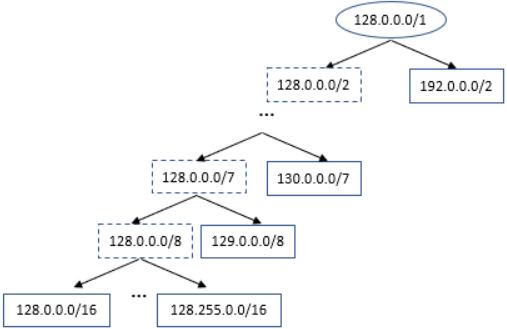
\includegraphics[width=\linewidth]{HHH/jpg_figures/sa_vs_htf.JPG}
\caption{The frontier after retraction in \ref{algo:htf} and \ref{algo:sa} with a single interesting flowset.}
\label{fig:sa_vs_htf}
\end{figure}

\begin{algorithm}\small
    \SetKwInOut{Input}{Input}
    \SetKwInOut{Output}{Output}
    \Input{A stream of packets $S$, a threshold $\phi$, number of counters $C$ and the depth of the hierarchy $H$}
    \Output{set of HH and HHH in $S$}
    $F = init\_flowsets(C)$\;
    $levels=calculate\_levels(C,H)$\;
    $current\_level=levels[0]$\;
    $number\_rounds=|levels|$\;
    \ForEach{$r$ in $\{1..number\_rounds\}$}
    {
        $counters=assign\_counters(F)$\;
        $P=get\_round\_packets(r, number\_of\_rounds)$\;
        \ForEach{$counter$ in $counters$}{
            counter.value=$\sum\limits_{\{p\in P : flow(p)\in counter.flowset\}}value(p)$\;
        }
        \If{$r < number\_rounds$}
        {
            $l=levels[r]-current\_level$\;
            $to\_refine = calculate\_to\_refine(counters, F, current\_level)$\;
            $refined = refine\_flowsets(to\_refine,l)$\;
            $ancestors = \{\}$\;
            \ForEach{$f$ in $refined$}{
                $sa=calculate\_shared\_ancestor(f, F)$\;
                $ancestors.add(sa)$\;
            }
            $F=refined \cup ancestors$\;
        }
    }
    return $calculate\_hhh\_bottom\_up(\phi)$\; 
    \ignore{
    $hh\_per\_level=calculate\_hh\_per\_level(\phi)$\;
    $hhh\_per\_level=calculate\_hhh\_per\_level(\phi, hh\_per\_level)$\;
    return $hh\_per\_level, hhh\_per\_level$\;
    }
    \SetAlgoRefName{\saAlgo}
    \caption{}
    \label{algo:sa}
    \vspace{-0.1cm}
\end{algorithm}